\subsection{OpenMP}
As mentioned before the implementation used is the simple implementation. First the OpenMP was tested. Figure [Graph showing graph generation] shows a graph of the amount of time spent generating the graph as a function of the amount of cores that were assigned to the program. As can be seen in the graphs the time spent creating the graph linearly dependent on the amount of CPUs that can be used by the program. 

In figure [OPENMP GTEPS] it can be seen that the amount of lines that can be traversed does not rely on the amount of CPUs that are available to the process.

\subsection{MPI}
In figure \ref{} you can how the amount of TEPS increases as the number with the number of nodes. These results are from the experiments on the DAS-4. As the scale of the increases the the TEPS also increase up until a certain point. After this point the amount of TEPS decreases again. This can be seen for any  amount of nodes. There is always a tipping point where increasing the scale will not increase the amount of edges that can be traversed. In figure[nodes same the same can be seen but this figure shows it as a function of nodes. The larger the amount of nodes the more edges can be traversed. The only point where this is not true is at smaller scales, but the difference between the different nodes is very small on this small scale.

Comparing the results from the DAS-4 with the results from OpenNebula the same trends can seen. In figure [opennebula function of scale] it is shown that the amount of TEPS increases as the scale gets larger, up to a certain point, similar to the experiments on the DAS. The difference between the experiments is that the amount of TEPS is much smaller than the amount of TEPS that can be achieved on the DAS. On reason is that InfiniBand was not enabled on the OpenNebula. Im Figure[das as function scale without infi] the same experiments are shown as in  figure [das as function scale], but without the scale. On the DAS turning of  InfiniBand also has an effect on the performance, but it does not account for the still difference in the amount of edges that can be processed.

\begin{figure}
\centering
\begin{subfigure}{.5\textwidth}
  \centering
  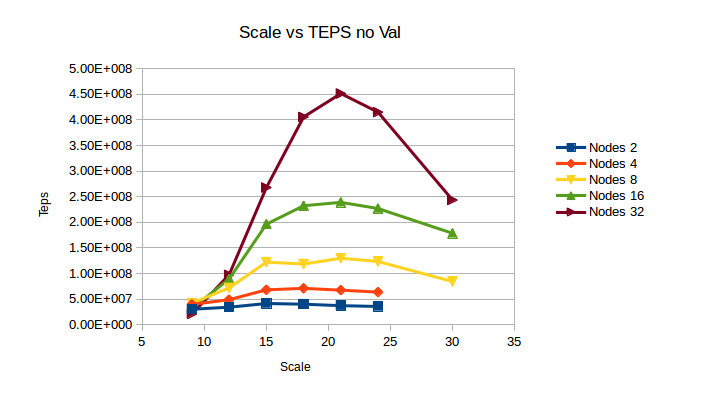
\includegraphics[width=\linewidth]{images/nodes_no_val.png}
  \caption{A subfigure}
  \label{fig:sub1}
\end{subfigure}%
\begin{subfigure}{.5\textwidth}
  \centering
  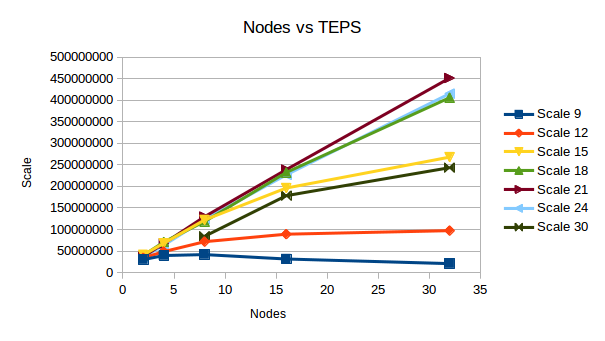
\includegraphics[width=\linewidth]{images/scales_no_val.png}
  \caption{A subfigure}
  \label{fig:sub2}
\end{subfigure}
\caption{A figure with two subfigures}
\label{fig:das_no_val}
\end{figure}


\subsection{Communication}

